







\section{Artificial Intelligence}

	\subsection{Definition:}
	Artificial intelligence (AI) is a new field of study that involves imitating human thinking in a machine it also refers to the simulation of human intelligence in machines that will be programmed to do tasks that would normally require the need of human intelligence, such as perception, reasoning, learning, and decision-making.\cite{russell2010artificial}.

	\subsection{Applications of Artificial Intelligence:}
		\paragraph{Natural language processing (NLP):}
		NLP is a field of AI that works on enabling machines to understand and interpret  the human language. NLP has many applications that can be used in normal day to day life like: language translation, chat bots, voice assistants and many other various jobs. \cite{christopher1999foundations}.

		\paragraph{Image recognition and computer vision:}
		AI-powered image recognition and computer vision technologies are  fields of technology that use algorithms to enable machines to interpret and understand visual data by classifying objects or patterns within the data and these technologies are used in a wide range of applications, including object detection, facial recognition, medical imaging, and autonomous vehicles. \cite{bishop2006pattern}.

		\paragraph{Predictive Analytic:}
		AI can be used to analyze large datasets and make predictions about future outcomes. Predictive analytic has applications in healthcare, finance, marketing, and many other fields. \cite{shmueli2010explain}.
	
\section{Machine Learning}
	\subsection{Definitions:}
		\paragraph{Definition 1:}
		Machine learning is a form of artificial intelligence that enables computers to learn from data without being programmed explicitly. The primary aim of machine learning is to allow computers to improve their performance on a specific task, such as recognizing images or speech, by analyzing large amounts of data and detecting patterns and trends. This involves the development of algorithms that can learn from the data, make predictions, or decisions based on that data, and create systems that can adapt and enhance their performance over time. The ultimate goal of machine learning is to enable computers to learn and make decisions in a way that simulates human intelligence. \cite{alpaydin2010introduction}.
		\paragraph{Definition 2:}
		Machine learning is a scientific field within artificial intelligence that focuses on the development of algorithms and statistical models to enable computers to act without being programmed explicitly. Its main objective is to teach machines to learn from data and use that knowledge to make decisions or predictions. Machine learning algorithms use statistical techniques to automatically identify patterns and trends in data and use them to make predictions or decisions about new data. This technique has been successfully implemented in numerous domains, such as image and speech recognition, natural language processing, predictive analytic, and self-driving cars, among others. \cite{murphy2012machine}.
		
	\subsection{Features of machine Learning}	
		\paragraph{Automation:}
		Machine learning automates the process of building analytical models. Once trained, a model can be used to make predictions or decisions without human intervention. This means that the system can learn patterns and relationships from data and make decisions based on that learning. The automated nature of machine learning makes it an efficient tool for tasks that require repetitive pattern recognition or analysis. Machine learning models can also be used to automatically detect and diagnose faults in complex systems, such as industrial equipment, by analyzing sensor data. \cite{alpaydin2010introduction}
	
		\paragraph{Adaptivity:}
		Machine learning models can adapt to changing data and learn from new examples. This means that they can improve their accuracy over time and become more effective. As new data becomes available, the model can be updated and retrained to improve its predictions. This adaptability is a key feature of machine learning, as it allows the system to continually learn and evolve to better meet the needs of its users. Machine learning models that can adapt to new data can be used in a wide range of applications, including fraud detection, speech recognition, and autonomous vehicles.  \cite{hastie2009elements}
	
		\paragraph{Generalization:}
		: Generalization is a key aspect of machine learning, which enables models to make predictions on new and unseen data by learning from the training data. The ability to generalize allows machine learning models to identify and apply patterns and relationships in the training data to new, unseen data. This is crucial because models may need to be applied to real-world situations where the training data is unavailable. For example, a machine learning model trained on historical sales data can be used to make predictions about future sales, even if the specific sales data is unknown. The ability to generalize is an important feature of machine learning as it allows models to be utilized in various applications, leading to improved accuracy and efficiency in making predictions and decisions. \cite{bishop2006pattern}
	
		\paragraph{Interactivity: }
		One of the key advantages of machine learning algorithms is their ability to interact with their environment and adapt their behavior in response to feedback. This means that machine learning systems can learn from their users and improve their performance over time. Interactive machine learning systems have a broad range of applications, including virtual assistants, chatbots, and recommendation engines. These systems can learn from user feedback and adjust their recommendations or responses to better satisfy the user's needs. This feature of machine learning is highly beneficial, as it enables the development of intelligent systems that can provide more personalized and accurate recommendations, leading to enhanced user satisfaction. \cite{amershi2014power}
	
		\paragraph{Scalability: }
		Machine learning algorithms are highly scalable, making them suitable for a wide range of applications that involve complex problems and large datasets. This scalability enables machine learning algorithms to be used in areas such as personalized recommendations, fraud detection, and medical diagnosis. The ability to handle large datasets is critical to machine learning as it allows algorithms to learn and make more accurate predictions. The scalability of machine learning models makes them highly versatile and applicable in various fields, including image recognition and natural language processing, where large datasets are crucial for model training and improved performance. \cite{jordan2015machine}
		
		\paragraph{Nonlinearity: }
		Machine learning models are designed to capture complex and often nonlinear relationships between input and output variables, making them highly effective for tasks such as natural language processing and image recognition. Nonlinearity refers to relationships between input and output variables that are not simple or linear, and instead are complex and nonlinear. Machine learning models excel at capturing these complex relationships, which can be used to make highly accurate predictions. For instance, a machine learning model used for image recognition can identify intricate features in an image, such as edges, textures, and colors, to classify it accurately. This feature of machine learning is critical for complex and challenging tasks that require advanced pattern recognition and analysis. \cite{lecun2015deep}
		
		
\section{Deep Learning}
	\subsection{Definitions}
			\paragraph{Definition 1:}
				Deep learning is a field of machine learning that utilizes artificial neural networks with multiple layers to extract complex features and patterns from data. By processing data through a hierarchical system of artificial neurons, deep learning models can identify and learn intricate relationships within the data, making it particularly useful for tasks such as image recognition, speech recognition, and natural language processing \cite{goodfellow2016deep}
			\paragraph{Definition 2:}
			Deep learning is a type of artificial intelligence that trains computers to improve their performance on a task by analyzing and adjusting their internal parameters. By using a layered approach to data processing, each layer of a deep neural network learns to extract progressively more complex features from the data, resulting in more accurate predictions and better generalization to new inputs. Deep learning has demonstrated remarkable success in various fields, such as image and speech recognition, natural language processing, and predictive modeling  \cite{lecun2015deep}
			
	\subsection{Applications :}
			\paragraph{Image Recognition :}
				Deep learning models can be trained to recognize objects in images and classify them into different categories. This technology has been used for facial recognition, object detection, and image segmentation, among other things. One such example is the use of convolutional neural networks (CNNs) for image recognition, which has shown great success in applications like self-driving cars and medical imaging. \cite{krizhevsky2017imagenet}
			
			\paragraph{Natural Language Processing (NLP):}
				Deep learning models can be used for language modeling, sentiment analysis, language translation, and many more NLP applications. For instance, deep learning models like recurrent neural networks (RNNs) have been applied to machine translation tasks, while transformer models such as BERT have been applied to tasks like question answering and sentiment analysis.  \cite{vaswani2017attention}
			\paragraph{Speech Recognition: }
				Deep learning models can be used for speech recognition tasks, including voice recognition, speaker identification, and speech-to-text conversion. Deep neural networks such as long short-term memory (LSTM) networks have been used to build robust speech recognition models. \cite{graves2005framewise}
			
			\paragraph{Autonomous Systems:}
				Deep learning has been applied to develop autonomous systems such as self-driving cars, drones, and robots. Deep reinforcement learning algorithms have been used to enable robots to learn how to perform tasks through trial and error. 	\cite{mnih2015human}
				
\section{Model Learning Methods and CNN}
		\subsection{CNN Definition :}
		A Convolutional Neural Network (CNN) is a type of deep learning model that has proven to be particularly effective in image classification tasks. It works by applying a series of convolutional filters to the input image, which helps to identify and extract meaningful features from the image. These features are then processed through a series of layers, allowing the network to learn increasingly complex representations of the image. The end result is a set of predicted classes or labels that describe the content of the input image. \cite{lecun2015deep}
	%	Reference: LeCun, Y., Bengio, Y., & Hinton, G. (2015). Deep learning. Nature, 521(7553), 436-444.
		
		
		\subsection{how CNN Works:}
		Convolutional Neural Networks (CNNs) are a type of deep learning model used in computer vision tasks, such as image classification, object detection, and segmentation. These models automatically extract important features from input images by applying convolutional filters.
		
		When processing an input image, a CNN uses these filters to detect patterns by sliding over the image and computing dot products between the filter weights and image pixels within the filter's receptive field. Afterward, the resulting feature maps are passed through activation and pooling layers to reduce their spatial resolution and into fully connected layers to classify the image.
		
		During the training process, CNN weights are updated using backpropagation and gradient descent to minimize the difference between the predicted output and the actual output. This allows the model to learn increasingly complex representations of the input image, enabling it to accurately recognize patterns and objects within images. Due to their impressive performance in various computer vision tasks, CNNs are commonly used in the field.
		
		\begin{figure}[h]
			\centering
			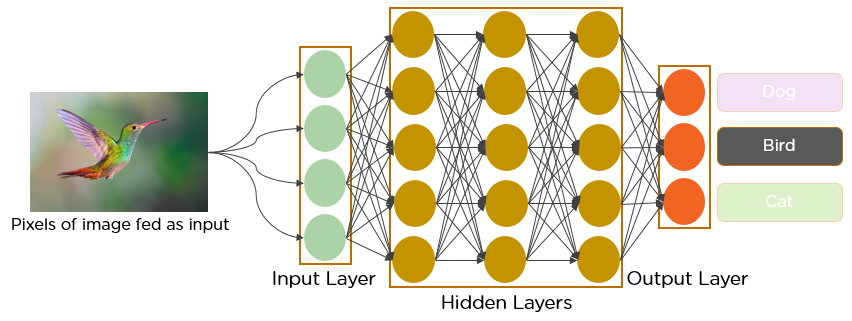
\includegraphics[width=0.8\linewidth]{images chap1/cnnimage.png}
			\caption{How CNN Algorithm Works}
			\label{cnnimage}
		\end{figure}
		
		
		
		\subsection{Learning Methods: }
			\paragraph{Supervised Learning}
			Supervised learning is a machine learning technique where the model is trained on labeled data, enabling it to learn to map input data to output data. This technique is commonly used in tasks such as image classification, speech recognition, and natural language processing. In supervised learning, the labeled data is used to train the model, and the trained model can then make predictions on new, unlabeled data. \cite{alpaydin2010introduction}
		
			\paragraph{Unsupervised Learning}
			Unsupervised learning is a machine learning technique where the model is trained on unlabeled data to find patterns or structure in the data. This technique is commonly used in clustering, dimensionality reduction, and anomaly detection, where the model groups similar data points together based on their similarities or differences. Unlike supervised learning, unsupervised learning does not rely on specific output data to guide the learning process. \cite{goodfellow2016deep}
		%	Goodfellow, I., Bengio, Y., & Courville, A. (2016). Deep Learning (1st ed.). MIT Press.
			\paragraph{Reinforcement Learning}
			Reinforcement learning is a machine learning technique where an agent learns by exploring its environment and receiving feedback. The goal of the agent is to maximize a cumulative reward signal by making decisions that lead to positive outcomes. This approach is commonly used in robotics and game playing, where the agent needs to learn through trial and error. \cite{sutton2018reinforcement}
		%	Sutton, R. S., & Barto, A. G. (2018). Reinforcement Learning: An Introduction (2nd ed.). MIT Press.
			\paragraph{semi-supervised Learning}
			This approach lies between supervised and unsupervised learning, and combines the benefits of both, the model can learn more efficiently and effectively 
			\paragraph{active learning}
			In active learning, the machine learning algorithm selects and queries the user for the most useful data points to label, rather than labeling all data points upfront. This method allows the algorithm to iteratively improve its model's performance, ultimately reducing the amount of labeled data required for training. Active learning is a useful technique in scenarios where labeled data is scarce or expensive to obtain, allowing for more efficient and effective use of resources. \cite{settles2009active}
			%Settles, B. (2009). Active Learning Literature Survey. Computer Sciences Technical Report 1648, University of Wisconsin-Madison.
			\paragraph{transfer learning.}
			Transfer learning is a method of reusing a pre-trained machine learning model's knowledge to solve a different but related problem. The technique involves fine-tuning the pre-trained model using a smaller dataset for the new task. By leveraging the learned features from the original task, the model can achieve better accuracy on the new task than it would without transfer learning.
			\cite{pan2010survey}
			%Pan, S. J., & Yang, Q. (2010). A survey on transfer learning. IEEE Transactions on knowledge and data engineering, 22(10), 1345-1359.
			\begin{figure}[h]
				\centering
				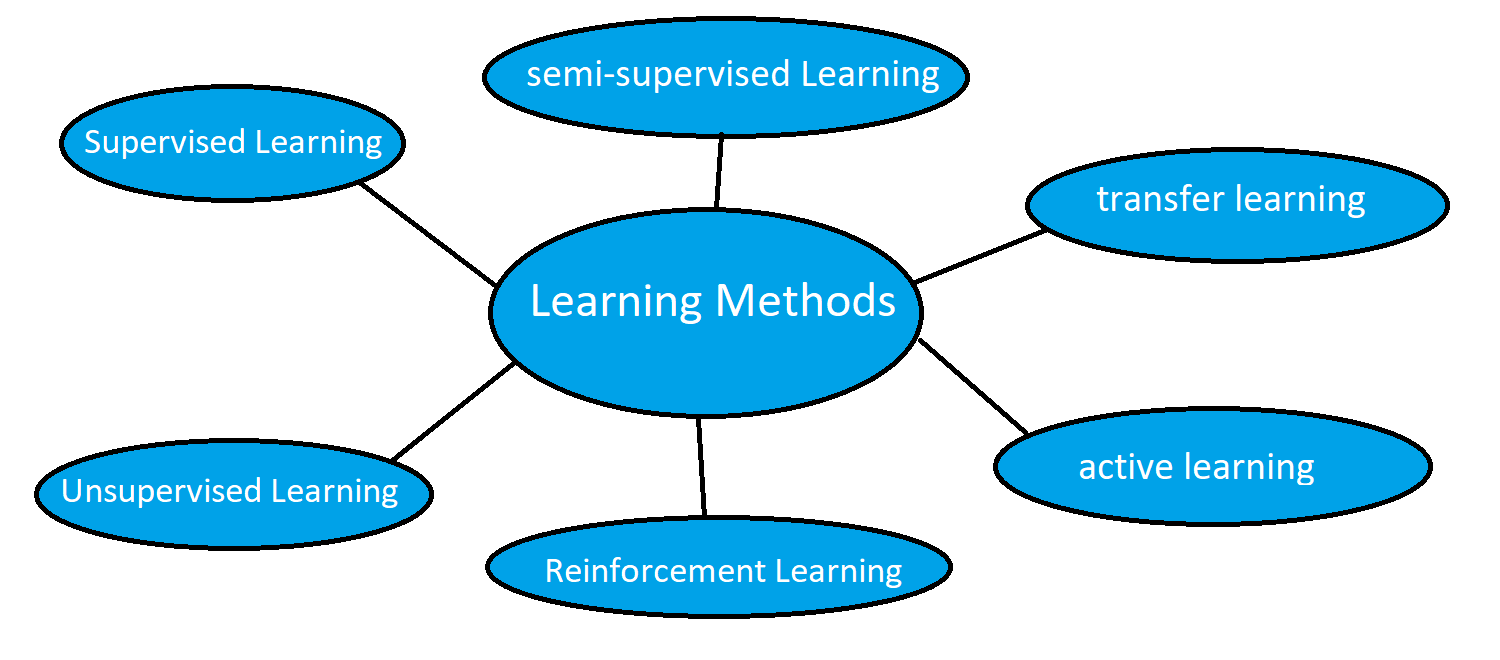
\includegraphics[width=0.8\linewidth]{images chap1/methods.png}
				\caption{Model Learning Methods}
				\label{methods}
			\end{figure}
			
		%	\bibliographystyle{unsrt}
		%	\bibliography{ref}	
		%	\listoffigures
